\section{Class 18}

\subsection{Distribution of residuals}

\begin{result}
    \textbf{Residuals are normally distributed}. 
    \begin{align*}
        \bm{E} \sim N_n \left( \bm{0}, \sigma^2 \left( \bm{I} - \bm{P_X} \right)  \right) 
    \end{align*}
\end{result}

\begin{proof}
    \textbf{Normality}: Since $\bm{Y} \sim N_n \left( \bm{X \beta}, \sigma^2 \bm{I} \right) $, and $\bm{E} = (\bm{I} - \bm{P_X}) \bm{Y}$, $\bm{E}$ is a linear combination of normals.  \\

    \textbf{Zero mean}: 
    \begin{align*}
        \mathbb{E}\left[ \bm{E}\right]  &= \mathbb{E}\left[ \bm{Y} - \hat{ \bm{Y}}\right]  \\
        &= \mathbb{E}\left[ \left( \bm{I}- \bm{P_X} \right) \bm{Y} \right]  \\
        &= \left( \bm{I} - \bm{P_X} \right)  \mathbb{E}\left[ \bm{Y}\right]  \\
        &= \left( \bm{I} - \bm{P_X} \right) \bm{XP} \\
        &= \bm{X \beta} - \bm{P_X} \bm{X \beta} \\
        &= 0
    \end{align*}

    \textbf{Variance}: 
    \begin{align*}
        Var ( \bm{E}) &= Var \left( ( \bm{I} - \bm{P_X}) \bm{Y} \right)  \\
        &= \sigma^2 \left( \bm{I} - \bm{P_X} \right)^2 \\
        &= \sigma^2 \left( \bm{I} - \bm{P_X} \right) 
    \end{align*}
\end{proof}

\subsubsection{Estimating $\sigma^2$ in MLR} 

\begin{definition}
    (Sum of square error, SSE): The \textbf{SSE} is defined as 
    \[
        \bm{E}^{\top}\bm{E} = \sum\limits_{i = 1}^{n}  (Y_i - \hat{Y}_i)
    \]
\end{definition}

\begin{result}
    The SSE follows a \textit{chi-squared} distribution with $n - (p + 1)$ degrees of freedom. \\
    \[
        \bm{E}^{\top}\bm{E} \sim \sigma^2 \chi_{n - (p + 1)}
    \]
\end{result}

\begin{result}
    An \textbf{unbiased estimate} of $\sigma^2$ is 
    \begin{align*}
        \hat{\sigma}^2 = \frac{ SSE}{n - (p + 1)} = \frac{\bm{E}^{\top}\bm{E}}{n - (p + 1)}
    \end{align*}
\end{result}

\begin{result}
    Facts about the eigenvalues of $\bm{I} - \bm{P_X}$ 
    \begin{enumerate}
        \item $\rank(\bm{X}) = p + 1 \implies \rank(\bm{P_X}) = p + 1$
        \item Since $(\bm{I} - \bm{P_X})$ idempotent, it has eigenvalues of 0 or 1 
        \item $\bm{P_X}$ has $p+1$ eigenvalues 1 and $n- (p + 1)$ eigenvalues $0$ 
        \item $(\bm{I - \bm{P_X}})$ has $n - (p + 1)$ eigenvalues 1 and $p + 1$ eigenvalues $0$.
    \end{enumerate}
\end{result}


\begin{proof}
We express $\bm{E} = \left( \bm{I} - \bm{P_X} \right)^{ \frac{1}{2}} \bm{\eta} $, where $\bm{\eta} \sim N_n \left( \bm{0}, \sigma^2 \bm{I} \right) $. Then 
\[
    \bm{E}^{\top}\bm{E} = \bm{\eta}^{\top} \left( \bm{I} - \bm{P_X} \right) \bm{\eta}
\]
By spectral theorem, 
\begin{align*}
    \bm{I} - \bm{P_X} &= \bm{UD}  \bm{U}^{\top}
\end{align*}
Where 
\[
    \bm{UU}^{\top} = \bm{U}^{\top}\bm{U} = \bm{I}
\]
And 
\[
    \bm{D} = \begin{pmatrix} 
      \bm{I}_{n - (p + 1) \times n - (p + 1)} & \bm{0} \\
      \bm{0} & \bm{0}
    \end{pmatrix}
\]
Also note that 
\begin{align*}
    \bm{U}^{\top} \bm{\eta} \sim N_n \left( \bm{0}, \sigma^2 \bm{U}^{\top} \bm{U} \right)  = N_n \left( \bm{0}, \sigma^2 \bm{I} \right) 
\end{align*}
Hence 
\begin{align*}
    \bm{E}^{\top} \bm{E} &= \bm{\eta}^{\top} \left( \bm{I} - \bm{P_X} \right)  \bm{\eta} \\
    &= \bm{\eta}^{\top} \bm{U} \begin{pmatrix} 
      \bm{I}   & \bm{0} \\ \bm{0} & \bm{0}
    \end{pmatrix}
     \bm{U}^{\top} \bm{\eta} \\
     &= \bm{ \theta}^{\top} \begin{pmatrix} 
    \bm{I}   & \bm{0} \\ \bm{0} & \bm{0}
     \end{pmatrix}   \bm{ \theta}\\
     &= \sum\limits_{i = 1}^{n - (p + 1)}  \theta_i^2  \\
     & \sim \sigma^2 \chi^2_{n - ( p + 1)}
\end{align*}
\end{proof}


\subsection{Confidence interval and hypothesis testing for gression coefficients}

\begin{result}
    The residuals $\bm{E}$ and $ \hat{ \bm{ \beta}}$ are \textbf{independent}.
\end{result}
\begin{proof}
    Since $ \left( \hat{ \bm{ \beta}}, \bm{E} \right) $ normally distributed, suffices to show that 
    \[
        \operatorname{Cov}  \left( \hat{ \bm{\beta}}, \bm{E} \right)  = 0
    \]

    Since 
    \begin{align*}
        \hat{\bm{\beta}} &= \bm{AY}, \bm{A} = \left( \bm{X}^{\top} \bm{X} \right)^{-1} \bm{X}^{\top} \\
        \bm{E} &= \bm{BY}, \bm{B} = \bm{I - P_X}
    \end{align*}
    \begin{align*}
        \operatorname{Cov} (\bm{AY}, \bm{BY}) &= \sigma^2 \bm{AB} \\
        &= \sigma^2 \left( \bm{X}^{\top} \bm{X}  \right)^{-1} \bm{X}^{\top} \left( \bm{I - P_X} \right)   \\
        &= \sigma^2 \left( 
            \left( \bm{X}^{\top} \bm{X} \right)^{-1} \bm{X}^{\top}  -
            \left( \bm{X}^{\top} \bm{X} \right)^{-1} \bm{X}^{\top} \bm{X} \left( \bm{X}^{\top} \bm{X} \right)^{-1} \bm{X}^{\top} 
         \right)  \\
        &= \sigma^2 \left( 
            \left( \bm{X}^{\top} \bm{X} \right)^{-1} \bm{X}^{\top}  -
            \left( \bm{X}^{\top} \bm{X} \right)^{-1} \bm{X}^{\top}
         \right)  \\
        &= \bm{0}
    \end{align*}
\end{proof}


\begin{result}
    Since $\hat{ \bm{\beta}}$ and $\hat{ \sigma^2}$ indepdenent, where
    \[
        \hat{ \bm{\beta}} \sim N_{p + 1} \left( \bm{\beta}, \sigma^2 \left( \bm{X}^{\top} \bm{X} \right)^{-1}  \right) 
    \]
    and 
    \[
        \hat{ \sigma^2} = \frac{SSE}{n - (p + 1)} \sim \frac{\sigma^2 \chi_{n - (p + 1)}^2}{n - (p + 1)}
    \]
    Therefore, for $0 \leq i \leq p$
    \begin{align*}
        \frac{\hat{\beta}_i - \beta_i}{ \hat{ \sigma} \sqrt{ \left( \bm{X}^{\top} \bm{X} \right)^{-1}_{ii} }} \sim t_{n - (p + 1)}
    \end{align*} 

    \textbf{Confidence interval for $\beta_i$} The following is a $100(1- \alpha)\%$ confidence interval for $\beta_i$
    \[
        \left[ \hat{\beta}_i \pm t_{n - (p + 1), \frac{\alpha}{2}} \hat{\sigma} \sqrt{(\bm{X}^{\top}\bm{X})^{-1}_{ii}} \right] 
    \]

    \textbf{Hypothesis testing}: to test 
    \[
        H_0: \beta_i = 0 \text{ vs } H_1: \beta_i \neq 0
    \]
    at level $\alpha$,
    
    We reject $H_0$ when 
    \[
        \left| \frac{\hat{\beta_i}}{ \hat{\sigma} \sqrt{
            \left( \bm{X}^{\top}\bm{X} \right)^{-1}_{ii}
        }} \right|  > t_{n - (p + 1), \frac{\alpha}{2}}
    \]
\end{result}

\subsubsection{F-test and ANOVA}

The MLR model is
\[
    y_i = \beta_0 + \beta_1 x_{1i} + \hdots \beta_p x_{p_i} + \epsilon_i
\]

How well does the least squares model fit the data? \\

We test 
\[
    H_0: \beta_1 = \beta_2 = \hdots = \beta_p = 0 \text{ vs } H_1: \beta_i \neq 0 \text{ for some } 1 \leq i \leq p
\]

Under $H_0$, the model is 
\[
    y_i = \beta_0 + \epsilon_i
\]
Hence
\[
    \hat{\beta}_0 = \bar{Y} 
\]

\begin{definition}
    (Sum of squares total, SST): The \textbf{SST} is defined as 
    \begin{align*}
        SST &= \sum\limits_{i = 1}^{n}  (y_i - \bar{Y} )^2 \\
        &= \bm{Y}^{\top} \left( \bm{I - P_{1}} \right) \bm{Y}
    \end{align*}
    Where $\bm{P_1}$ is the projection matrix on to the column space of $\bm{1}$ 
    \[
        \bm{P_1} = \bm{1} \left( \bm{1}^{\top} \bm{1} \right)^{-1} \bm{1}^{\top} = \frac{\bm{1}\ \bm{1}^{\top} }{n}
    \]
\end{definition}

\begin{definition}
    (Multiple $R^2$, coefficient of determinant): The $R^2$ or coefficient of determinant is defined as the proportion by which the LS model reduces the total sum of squares
    \begin{align*}
        R^2 &= 1 - \frac{SSE}{SST} \\
        &= \frac{SST - SSE}{SST}
    \end{align*}
\end{definition}

\begin{definition}
    (Adjusted $R^2$): The adjusted $R^2$ accounts for the fact that $R^2$ increases as more variables are added to the model. The adjusted $R^2$ is denoted 
    \[
        \bar{R}^2 = 1 - \frac{SSE / (n - (p + 1))}{SST / (n-1)} = 1 - \frac{SSE}{SST} \frac{n-1}{n-(p + 1)}
    \]
\end{definition}

\begin{definition}
    (SSR, Sum of squares regression): The \textbf{SSR} is defined as 
    \begin{align*}
        SSR &= SST - SSE \\
        &= \bm{Y}^{\top} \left( \bm{I - P_1} \right) \bm{Y} - \bm{Y}^{\top} \left( \bm{I - P_X} \right)  \bm{Y} \\
        &= \bm{Y}^{\top} \left( \bm{P_X - P_1} \right)  \bm{Y}
    \end{align*}
\end{definition}

\begin{result}
    Under $H_0$, SSR follows a \textit{chi-squared} distribution and is independent of SSE. \\
    \[
        SSR \overset{H_0}{\sim}  \sigma^2 \chi_p^2
    \]
    Therefore 
    \[
        F = \frac{SSR / p}{SSE /n - (p + 1)} \overset{H_0}{\sim}  F_{p, n-(p + 1)}
    \]
    And a level $\alpha$ test for goodness of fit (Hypothesis test in section 12.8.1) rejects $H_0$ when 
    \[
        F > F_{p, n- (p + 1), \alpha}
    \]
\end{result}

\begin{proof}
    Define matrix $\bm{W}$, 
    \begin{align*}
        \bm{W}:&= \left( \bm{P_X - P_1} \right)^{ \frac{1}{2}} \bm{Y} \\
        &= \left( \bm{P_X - P_1} \right)  \bm{Y} \\
        \overset{H_0}{\sim}  N \left( \bm{0}, \sigma^2 \left( \bm{P_X - P_1} \right)  \right) 
    \end{align*}
    Where $\bm{P_X - P_1}$ is the orthogonal projection matrix onto $\sigma \left( \{ \bm{x}_1, \bm{x}_2, \hdots \bm{x}_p \}  \right) $. \\

    Under $H_0$ 
    \begin{align*}
        \mathbb{E}\left[ \bm{Y}\right]  = \beta_0 \bm{1} \perp \sigma \left( \{ \bm{x}_1, \hdots \bm{x}_p \}  \right) 
    \end{align*}
    The matrix $\bm{P_X - P_1}$ has $p$ eigenvalues 1 and $n-p$ eigenvalues 0. Hence 
    \[
        SSR = \bm{W}^{\top} W \sim \sigma^2 \chi_p^2
    \]
    To show $SSR \perp SSE$, it suffices to show 
    \[
        \operatorname{Cov}  \left( \bm{E}, \bm{W} \right)  = 0 
    \]
    \begin{align*}
        \operatorname{Cov} \left( \bm{E}, \bm{W} \right)  &= \sigma^2 \left( \bm{I - P_X} \right)  \left( \bm{P_X - P_1} \right)  \\ 
        &= \bm{P_X} - \bm{P_1} - \bm{P_X} + \bm{P_X P_1} \\
        &= \bm{P_X P_1} - P_1 \\
        &= \bm{P_X} \frac{\bm{1}\ \bm{1}^{\top}}{n} - P_{\bm{1}} \\
        &= \frac{\bm{1}\ \bm{1}^{\top}}{n} - \bm{P_1} \text{ since } \bm{P_X 1 = 1} \\
        &= \bm{P_1} - \bm{P_1} \\
        &= \bm{0}
    \end{align*}
    
\end{proof}

\begin{center}
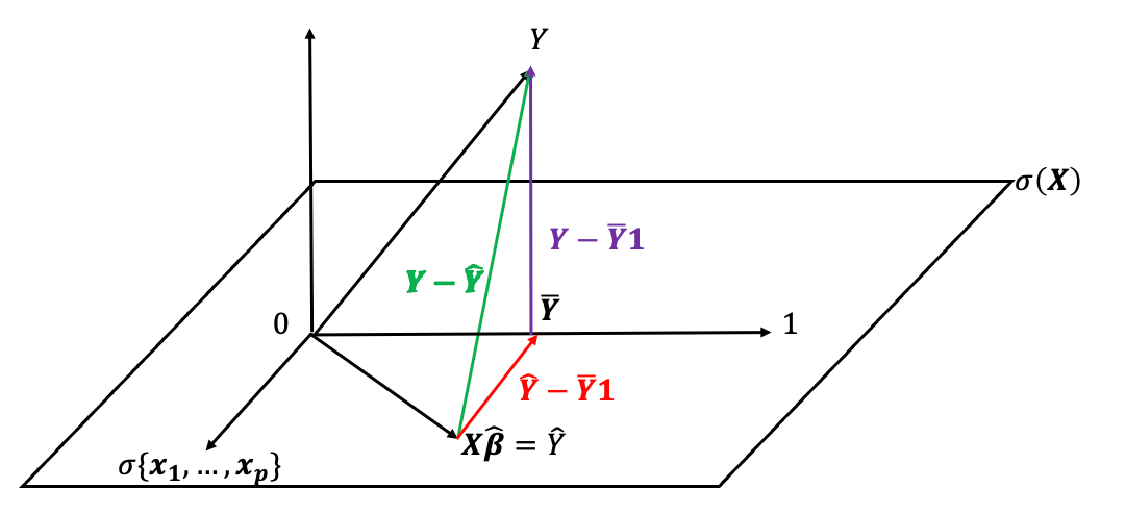
\includegraphics[width = 0.9\textwidth]{figures/fig_17_2.pdf}
\end{center}


\textbf{ANOVA Table}

\begin{center}
\begin{tabular}{c c c c}
    \textbf{Source} & \textbf{Sum of Squares} & \textbf{Degrees of Freedom} & \textbf{Mean Square / F-statistic} \\
    Regression & 
    $SSR = \bm{Y}^{\top} (\bm{P_X} - \bm{P_1}) \bm{Y}$ &
    $p$ &
    $\displaystyle \frac{SSR}{p}$ \\
    Error &
    $SSE = \bm{Y}^{\top} (\bm{I} - \bm{P_X}) \bm{Y}$ &
    $n - (p + 1)$ &
    $\displaystyle \frac{SSE}{n - (p + 1)}$ \\
    Total &
    $SST = \sum_{i=1}^{n} (y_i - \bar{Y})^2 = \bm{Y}^{\top} (\bm{I} - \bm{P_1}) \bm{Y}$ &
    $n - 1$ &
    \\
\end{tabular}
\end{center}

\newpage